% 3dprint.tex:

\chapter{3-D PRINTED PHANTOMS} % all caps please
\label{chap:3dprint}

\section{Introduction}
In order evaluate the performance of the NIR systems we have built, we need to use phantoms. Phantoms are physical samples carefully made to mimic the optical properties of human tissues\cite{Pogue2006}. By imaging these objects of known optical properties, we can evaluate the accuracy of a new system by comparing its result against existing systems. Creating these phantoms is complex: not only do you need create recipes that lead to the optical properties you want, phantoms must also be manufactures in specific geometries tailored to what the NIR system will measure. To address the optical properties, phantom makers tend to focus on mimicking the absorption coefficient ($\mu_a$) and the reduced scattering coefficient ($\mu_s^{'}$) of biological tissue~\cite{Dempsey2017} by using mixtures of scattering agents and absorbing pigments with a clear base~\cite{Hebden1995, Dong2015}. The shape of the phantom is typically created using traditional fabrication techniques, either mold casting~\cite{Hahn2012} or spin coating~\cite{Park2013}. 

Traditionally, as NIR imaging was in its infancy, these methods sufficed to create simple phantoms. However, these methods fall short in supporting complex geometries. As new NIR systems are developed to image the brain~\cite{Hebden2002, Villringer1997} and the breast, we will need to evaluate their performance with phantoms that have complex structural and physiological properties. While some phantom makers use intricate methods and procedures to develop geometrically complex phantoms~\cite{Mobashsher2014}, these phantoms take days to manufacture, require lots of equipment and expertise, and the manual process leads to  geometry and optical property variations due to human variability. Thus, to support the system development, calibration, and testing of new imaging methods~\cite{Cerussi2012, Diep2015} (like the NIR systems developed in this thesis), we need a new method to manufacture phantoms with spatially varying optical properties and anatomically accurate geometries.

Rather than add structure-generating methods to traditional phantom making, we propose a method to add customizable optical properties to a digital fabrication method that is already engineered to produce arbitrary geometry---fused deposition modeling (FDM). FDM is a form of 3-D printing that creates a 3-D object by adding solid material layer-by-layer~\cite{Dong2015}. While traditional 3-D printing uses a single filament material to generate a 3-D object, we proposed the mixing of grey (absorbing), white (scattering), and transparent (base) filament colors to produce the desired optical properties. 

The use of 3-D printing for phantom development allows for customizable properties using raw printing materials and the creation of spatially varying optical properties within a 3-D printed phantom. This allows the creation of a wide range of phantoms with precisely known optical properties, geometries, and inclusions of various resolutions (size, shape, depth). Most significantly, the design of a 3-D printed standardized calibration phantom for DOT minimizes geometry and optical property variations due to human variability. In this way, researchers can manufacture identical phantoms using in-situ materials with resolutions limited only by their 3-D printer, effectively allowing independent DOT systems to be characterized by the same exact phantom. 

In this Chapter we will detail our method to develop 3-D printed phantoms. We will first describe a workflow to characterize new filaments to account for variations in produced lots of the same color. We then show details of a slicer with the ability to slice an assembly of multiple STL files. The slicer is able to assign filament ratios (tissue profiles) to each individual STL, allowing the printer to adjust the mixing ratio of the extruder as it prints embedded inclusions into the large geometric print. To demonstrate the capabilities of the slicer, we will slice anatomical geometries with multi-tissue types for each of the three NIR systems in this study, including a finger with arteries for MOXI, a head phantom with spherical inclusions for use with MOBI, and a breast-shaped phantom with inclusions for OMCI. Finally, in order to encourage the use of our method, we will disclose a list of lessons learned to help others attempt to replicate our phantoms. 



\section{3-D Printing Hardware}
This project utilizes an experimental fused deposition modeling (FDM) multi-material 3-D printer (QuadFusion, M3D). This marlin-based printer has an extrusion bar-based frame and uses stepper motors to control motion. The extrusion head is composed of small stepper motors to guide four filaments through a metal nozzle with a polytetrafluoroethylene (PTFE) insert. The PTFE insert is a cylindrical piece with 4 milled out holes that extent from end to end. Mixing occurs in the nozzle tip. Due to the need to mix filaments into one nozzle exit, we used polyethylene terephthalate glycol (PETG) instead of the standard polylactic acid (PLA) filament. PLA is the most popular thermoplastic for 3-D printing because of its cost, ease of print (it is semi-flexible and very forgiving), and it does not off-gas any fumes. However, PLA is difficult to mix with other materials due to its limited temperature range. At high temperatures (above 200\textdegree~Celsius), it releases water which causes high pressure build up in nozzles. To resist the higher temperate and water, PETG is used. PETG is more viscous at higher temperatures, allowing it to easily fuse with other PETG filament. 


\section{New Filament Characterization}
The filament profiles are the derived settings used for a particular filaments. Although the majority of printing settings are consistent across PETG filaments, certain features must be accounted for, particularly, the extrusion multipliers and retraction amount. The extrusion multiplier (EM) is a setting used to account for variability in extrusion amounts. An extrusion multiplier of 1 means that 1 mm of filament is extruded for every 1 mm requested. Due to the filament path (the Bowden tube, motor teeth, varying temperatures), certain filaments in certain printers may require over or under extrusion to extrude the correct amount of filament. Retraction amount is the amount of filament to pull back up into the nozzle as the print head moves in between printing layers. When this value is too low, you will see ``stringing'' in prints from the oozing of material while the head is in motion. Too much retraction and the printer will not print the first few millimeters upon restarting since the nozzle is empty of filament.

To account for variations in manufactured filament of the same color by the same manufacturer, we have developed a method to characterize filaments and create filament profiles for each spool of filament. In fairness, the variability in extrusion multiplier is not entirely due to the manufacturer. The QuadFusion head is a complex head that requires filaments to be driven through curved paths and high pressure that result in friction. We calculate filament-specific EMs for each spool used in our printer by printing a square wall with the thickness of a single path width (PW). We then empirically determine the EM based on the desired path width and actual path width of the print. The steps are outlined in Figure~\ref{fig:emflowchart}.

\begin{figure}
	\begin{center}
	   \subfigure[]  {\label{fig:emflowchart}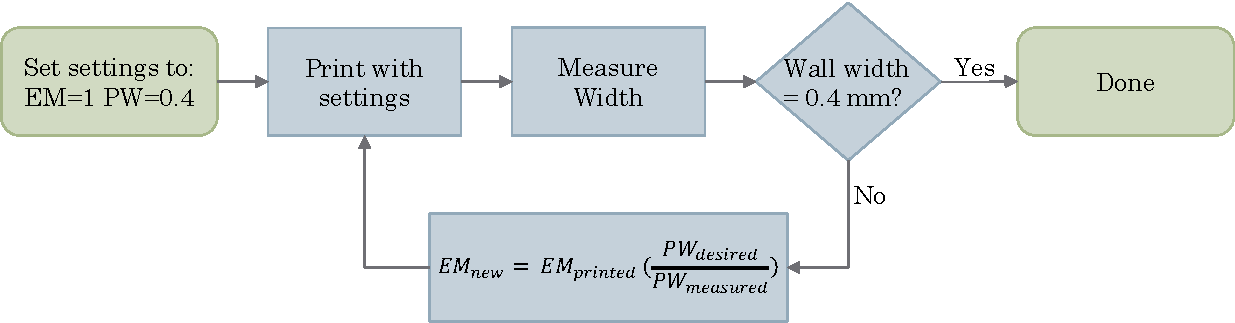
\includegraphics[width=\textwidth]{fig/3dprint/emflowchart.pdf}}
	   \subfigure[]{\label{fig:caliper}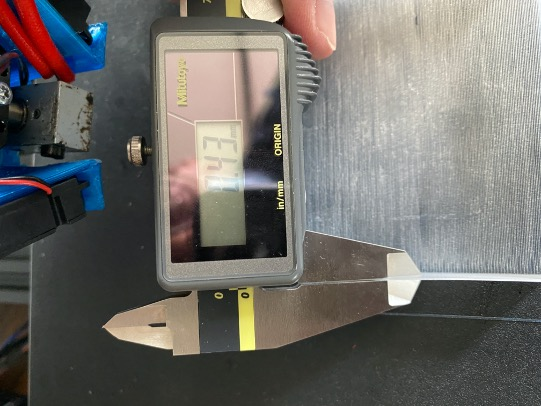
\includegraphics[width=.2\textwidth]{fig/3dprint/caliper.jpg}}
	   \subfigure[]{\label{fig:clear}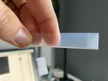
\includegraphics[width=.35\textwidth]{fig/3dprint/clear.jpg}}
	\end{center}
	\caption{} 
	\label{fig:em}
\end{figure} 

\begin{enumerate}
    \item First, set the EM=1 and the path width to 0.4 mm and print the square wall.
    \item Use calipers to measure the actual path width of the print.
    \item Use the actual path width and designed path width to determine a new EM using the formula $EM_{new} = EM_{printed} \times (PW_{desired}/PW_{measured})$
    \item Print the square wall again with the new EM and repeat steps 2 and 3 until the measured EM matches your desired EM. 
\end{enumerate}

A 3-D printed tissue type is a simply a mixing ratio of multiple characterized filament profiles. While one filament profile informs of the settings for printing a single filament, we have to create combined printing settings when mixing multiple filaments (tissue types). This is done as a weighted average of the settings scaled by the mixing ratios. For example, if white, grey, black, and clear filaments each have extrusion multipliers of 1, 0.98, 1, and 0.9, respectively, and we want to mix them in a 30/20/0/50 ratio, then the final extrusion multiplier would be
$(1\times30 + 0.98\times20 + 1\times0 + 0.9\times50) / (30+20+0+50) = 0.946$ Similarly, the extrusion motors are driven at scaled rates based on the filament mixing ratio.



\section{Multi-filament slicing}
\subsection{Artifacts for purging during transition}
One difficulty in fused multi-material 3-D printing not found in single filament printing is the need to purge the nozzle in between changing mixing ratios for different tissue types on the same layer. For example, if we want two separate mixing ratios for concentric rods, the nozzle needs to be purged in between printing the outside color and printing the inside color. Purging refers to the extrusion of sacrificial filament when the outputted mixed filament is transitioning between different two ratios (tissue types).

We have implemented a ``caging'' method in which a cage is built around the print to purge the nozzle. The method is an extension of the ``brim'' artifact commonly used to help prints adhere to the print bed. Essentially, at every layer, concentric shapes around the model are printed for each ratio. This allows the nozzle to fully transition to a new mixing ratio prior to continuing the print. This results in a cage around the print. 

\begin{figure}
	\begin{center}
	\subfigure[]{\label{fig:caging01}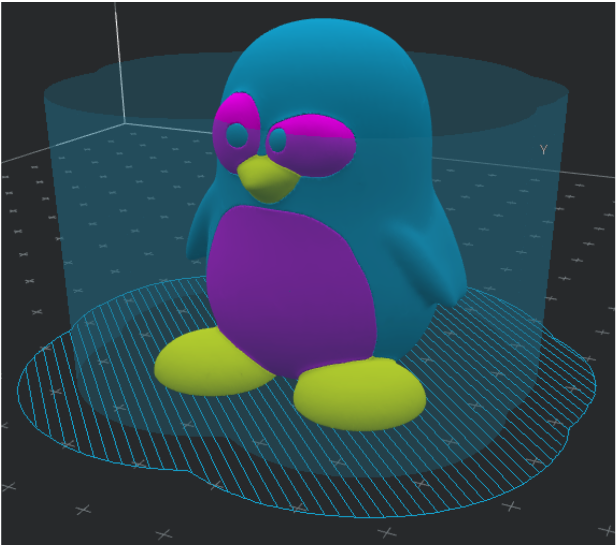
\includegraphics[height=4cm]{fig/3dprint/caging01.png}}
	\subfigure[]{\label{fig:caging02}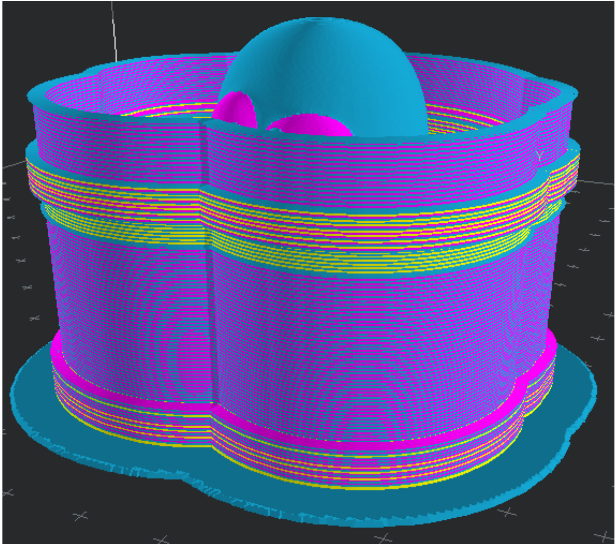
\includegraphics[height=4cm]{fig/3dprint/caging02.png}}
	\subfigure[]{\label{fig:caging03}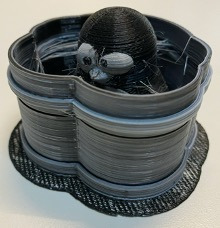
\includegraphics[height=4cm]{fig/3dprint/caging03.jpg}}
	\end{center}
	\caption{The ``caging'' purge method (a) An example penguin composed of three different tissue types. (b) The same print with the cage shown. The colors of the cage indicate the colors on that segment of the print. (c) Resulting 3-D printed penguin. } 
	\label{fig:caging}
\end{figure} 

\subsection{MOXI, MOBI, and OMCI system slicing}



\section{Lessons learned for use of PETG in filament mixing}
The use of PETG filament, a ``caging'' purging method, mixed filament ratio-based extrusion multipliers, and an experimental FDM 3-D printer has taught us many lessons. To facilitate future researchers in this space, here is a list of rule-of-thumbs and pitfalls to avoid. 

\begin{itemize}
    \item BED MATERIAL: PETG sticks very well to the bed. The use of sacrificial blue tape on the print bed will prevent you from buying new print beds when you can’t remove the print fully. \item LEVELING: Add a decent gap between nozzle and bed. Typical 3D printers level the bed by using a single sheet of regular printing paper as the unit of measure between the nozzle and the print bed. To account for the “gooey”-ness of PETG, use 3 pieces of paper.
    \item BED TEMP: Start bed temperature around 80°C. Don't go above 100°C (90°C is probably the highest). Higher is better for bed adhesion, but PETG already adheres pretty well. Consider lowering your nozzle before increasing the temperature. 
    \item NOZZLE TEMP: PETG prints between 230°C and 250°C. But PTFE, the white tube inside the nozzle, has a 250-260°C melting point, so don't print above 250°C.
    \item Start at 230°C and do some test prints. If you hear a knocking noise during printing, your extruder is skipping, and you should increase the nozzle temperature by 5°C. If still stringing, retract more.
    \item RETRACTION SPEEDS: Don’t go with high speeds for retraction PETG. Set the retraction speed to around 25 mm/s. Retraction distance should be set at about 3 or 4 millimeters for direct drive extruders. With PETG, retraction speed is more important than distance. If you still have oozing and stringing, try lowering the retraction speed.
    \item TRAVEL SPEED: One more parameter that will help in reducing oozing is the travel speed. PETG tends to drip from the tip of the nozzle, especially if the nozzle temperature is high. To combat this, try increasing the travel speed as high as possible.
    \item PRINT SPEED: PETG is very sensitive to print speed. Print too fast and you’ll have poor layer adhesion, extruder skipping, and low print quality—print too slow and you’ll end up with deformed parts, stringing, and oozing. You’ll have to find the sweet spot with the printer and filament you’re using. A good place to start is between 50-55mm/s. We suggest 25 mm/s for the first layer and the outer wall, while travel moves should be as fast as possible, at least 120 mm/s, to avoid oozing.
    \item FANS: We recommend printing without fans for the first layer or two, and then full fan after that. Fan ON is slightly worse adhesion, but better quality.
\end{itemize}


% --- EOF ---